\documentclass{article}
\usepackage[T1]{fontenc}
\usepackage{lmodern}
\usepackage{graphicx}
\usepackage{amsmath,amssymb}
\usepackage[a4paper,margin=2cm]{geometry}
\usepackage[absolute,overlay]{textpos}
\setlength{\TPHorizModule}{1mm}
\setlength{\TPVertModule}{1mm}
\usepackage[indonesian]{babel}
\usepackage{hyperref}
\setlength{\emergencystretch}{2em}
% unit: Halaman 32

\begin{document}

% === Halaman 32 (llm) ===

\begin{verbatim}
# Program utama

\vspace{127.71mm}

public_key, private_key = PembangkitanKunciRSA()

pesan = input("Ketikkan pesan teks: ")

ciphertext = encrypt_message(pesan, public_key)
print("\nCiphertext:", ciphertext.hex())

decrypted_message = decrypt_message(ciphertext, private_key)
print("\nPesan setelah dekripsi:", decrypted_message)
\end{verbatim}

% deskripsi: Screenshot potongan kode program Python untuk implementasi enkripsi dan dekripsi RSA.
% bbox normalisasi: [0.1100, 0.1400, 0.7800, 0.5700]
\begin{textblock*}{140.70mm}(23.10mm,41.58mm)
\noindent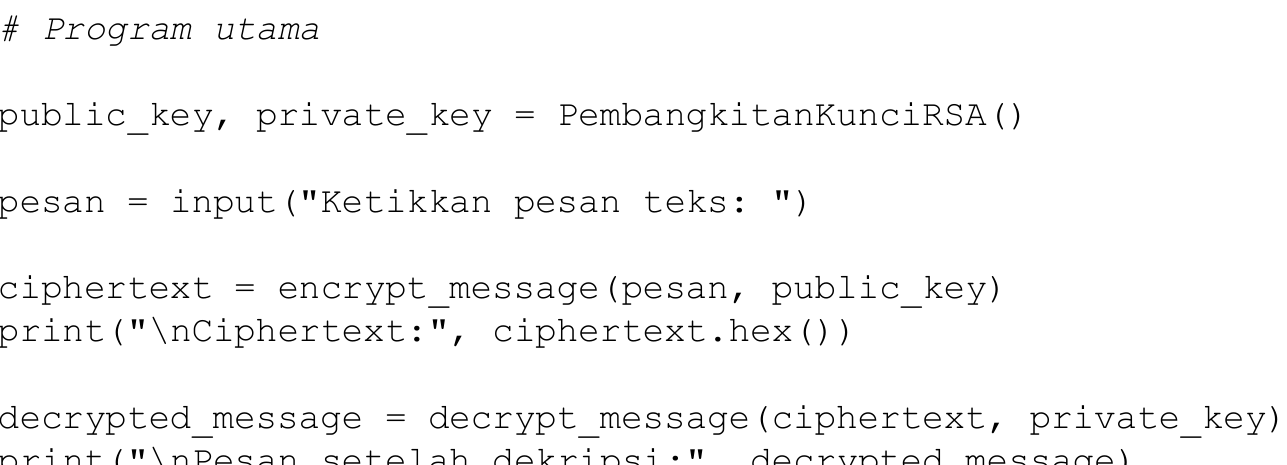
\includegraphics[width=140.70mm,height=127.71mm]{../../images/llm/page_032_img_01.png}%
\end{textblock*}

\end{document}
